\documentclass[11pt]{article}
\usepackage[margin=1in]{geometry}
\usepackage{graphicx}
\usepackage{booktabs}
\usepackage{hyperref}
\usepackage{amsmath}
\usepackage{enumitem}
\usepackage{float}
\usepackage{caption}
\usepackage{booktabs}
\usepackage{setspace}

% Header and footer
\usepackage{fancyhdr}
\pagestyle{fancy}
\fancyhf{}
\lhead{STAT3106 Final Project}
\rhead{Somin Lee}
\cfoot{\thepage}

% Hyperlink colors
\hypersetup{
    colorlinks=true,
    linkcolor=blue,
    citecolor=blue,
    urlcolor=blue
}

\begin{document}

\begin{center}
  {\LARGE \textbf{Predicting Emergency Department Visits with Weather in NYC}}\\[1em]
  {\large Somin Lee (sl5260)}\\
  {\small Columbia University, Applied Mathematics}\\
  {\small May 8, 2025}
\end{center}

\vspace{1em}
\noindent\textbf{Repository:} \url{https://github.com/sominlee1211/stat3106FinalProject}\\
\noindent\textbf{Repository:} \href{https://github.com/sominlee1211/stat3106FinalProject}{GitHub — stat3106FinalProject}
\vspace{1em}

\section{Introduction}

Weather and climate are fundamental determinants of human health, influencing the incidence, severity, and spread of respiratory illnesses.  Fluctuations in temperature, humidity, wind speed, and precipitation create environmental conditions that can exacerbate viral transmission, impair respiratory defenses, and drive seasonal epidemics of influenza‐like illness (ILI) and pneumonia.  Public health researchers have long documented correlations between cold snaps, low humidity, and spikes in emergency department (ED) visits for respiratory complaints; yet, most hospital systems remain largely reactive, scaling resources only after patient volumes begin to surge.  

During my volunteer rotations in the Bellevue Hospital Emergency Department, one of the busiest hospitals in New York City, I witnessed firsthand the logistical challenges posed by ILI and pneumonia cases.  Unlike many other patient populations, individuals presenting with these infections must often be cohorted in isolation rooms or treated with higher nurse‐to‐patient ratios to prevent the spread and ensure close monitoring.  While physical space in the ED is fixed and often strained, staffing levels can be adjusted on shorter notice provided administrators have advanced warning of an impending surge.

If it were possible to predict ED visit volumes for ILI and pneumonia two weeks in advance, hospital administrators could proactively adjust staffing rosters, secure appropriate isolation capacity, and streamline supply procurement which would ultimately reduce wait times, minimizing contagion risk, and protecting both patients and healthcare workers.  A weather‐driven predictive model offers a concrete tool to translate meteorological forecasts into actionable staffing plans, shifting the ED’s approach from reaction to anticipation.  

In this study, I ask: \textbf{Can I leverage publicly available daily weather data to forecast two‐week–ahead counts of ILI and pneumonia ED visits?}

The audiences are ED administrators and frontline healthcare teams. By demonstrating a reliable relationship between key weather variables and ED demand, I aim to empower these decision makers with a data-driven early-warning system that saves time, reduces uncertainty, and ultimately improves patient care during respiratory illness seasons.  


\section{Data Preparation and Extraction}

\subsection{Emergency Department Visits Data}
The raw dataset from OpenData was loaded and inspected for multiple extraction dates. I selected the snapshot from 12/05/2022 as it had the most complete coverage and dropped the \texttt{extract\_date} column. The visit \texttt{date} field was parsed into \texttt{YYYY-MM-DD} format.

\subsection{Exploratory Data Quality Checks}
Basic checks confirmed:
\begin{itemize}[nosep]
  \item Date range: 2020-03-01 to 2022-12-03.
  \item Unique Zip Codes: 177 (excluding placeholder 10000).
  \item No missing calendar days across the full date sequence.
  \item Full coverage of all 177 zipcodes for every date.
\end{itemize}

\subsection{Geospatial Feature Generation}
I performed a reverse lookup of Zipcode to latitude/longitude using \texttt{zipcodeR}, generating \texttt{lat, lng} for each zipcode and exporting to \texttt{lat\_lon\_list.csv}.

\subsection{Weather Data Acquisition}

To build and deploy a two‐week–ahead ED visit forecast, I need both \emph{historical observed} weather (for model training) and \emph{future forecast} weather (as model inputs when predicting).  I therefore fetched:

\begin{enumerate}[nosep]
  \item \textbf{Historical archive data} (\texttt{/archive} endpoint):  
    Observed daily values from March 1, 2020 to December 6, 2022.  
    These actual measurements (temperature, precipitation, wind, radiation, etc.) form our training features, enabling the model to learn true weather–ILI relationships.
  \item \textbf{Forecast data} (\texttt{/forecast} endpoint):  
    16‐day meteorological predictions corresponding to each ZIP location.  
    At deployment time, these forecasts become the model’s \emph{input features} to predict ED visit volumes two weeks in advance.
  \item The 178 NYC zip codes were split into batches of 10 to respect API rate limits, and used a custom \texttt{safe\_get()} wrapper to automatically retry on HTTP 429 (“Too Many Requests”).
  \item Each batch’s archive and forecast responses were parsed, combined into an RDS file, and finally merged into \texttt{weather\_data\_all\_archiveANDforecast.csv}.
\end{enumerate}

\subsection{Dataset Dimensions and Sources}

\begin{itemize}[nosep]
  \item \textbf{Emergency Department visits:}  
    Raw extract from NYC OpenData (managed by NYC DOH), with
    \(\dim(\texttt{ed}) = 176{,}862\times5\)  
    (zip code, date, total visits, ILI/pneumonia visits, admissions).
  \item \textbf{Weather records:}  
    Historical archive + 16-day forecasts from Open-Meteo API, with\\
    \(\dim(\texttt{weather}) = 181{,}248\times18\)  
    (zip, date, 14 meteorological variables, source flag, etc.).
\end{itemize}

\section{Model Selection}

Figure~\ref{fig:corrplot} shows the pairwise correlations among ED visit counts and weather features.  Strong multicollinearity is evident, particularly among temperature metrics (mean, max, min), apparent temperature, and related radiation variables.

\begin{figure}[]
  \centering
  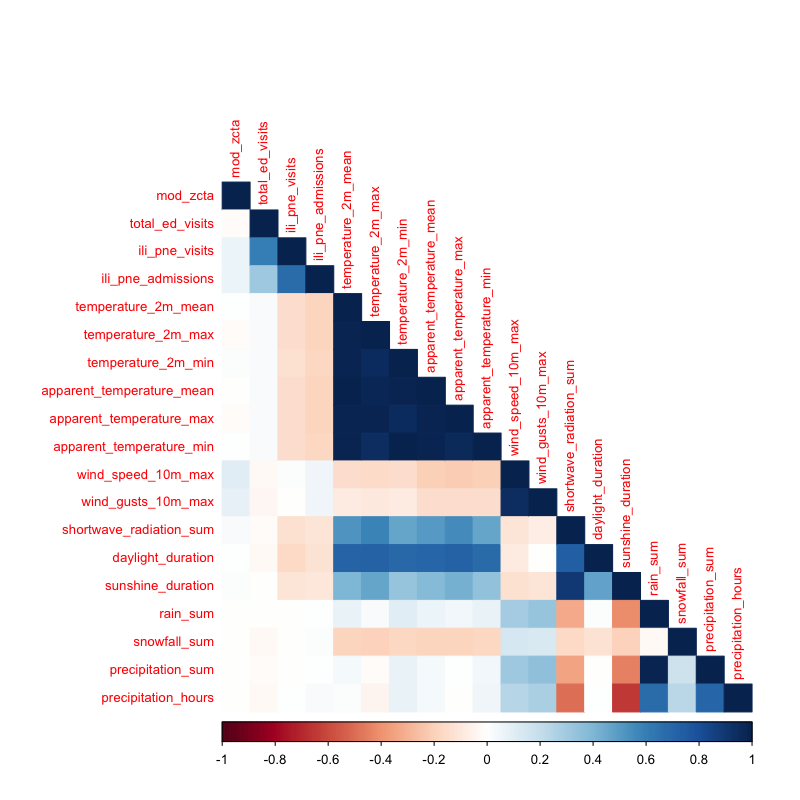
\includegraphics[width=1\textwidth]{corrplot.png}
  \caption{Correlation matrix of ED visit counts and weather predictors.}
  \label{fig:corrplot}
\end{figure}

Multicollinearity can destabilize coefficient estimates in linear models and impede interpretability.  Moreover, ED visit volumes likely depend on nonlinear interactions. For example, intuitively, combinations of low temperature, high wind speed, and low humidity may jointly increase respiratory stress more than each factor alone.  

To address these challenges, I selected the random forest model for its ability to:
\begin{itemize}[nosep]
  \item Handle correlated predictors without requiring explicit decorrelation or dimensionality reduction.
  \item Capture complex, nonlinear interactions among multiple features (e.g., \emph{cold + wind}).
  \item Provide robust out-of-sample performance via ensemble averaging and built-in cross-validation (via out-of-bag error).
\end{itemize}

Random forest balanced predictive accuracy, interpretability (via permutation importance), and computational efficiency, making it the most practical choice for an operational ED forecasting tool.

\section{Model Evaluation and Rationale}

\subsection{Random Forest Implementation with \texttt{ranger}}

I implement our predictive model using the \texttt{ranger} package in R, which provides a fast, memory‐efficient C++ implementation of Random Forest algorithm.  I choose \texttt{ranger} over the original \texttt{randomForest} package because \texttt{ranger} builds trees in parallel and handles large datasets (here, with 170,000+ rows) more quickly then \texttt{randomForest}.

\subsection{Out‐of‐Bag (OOB) Error}

Out‐of‐bag error is estimated by, for each tree, predicting only on those samples \emph{not} used to build that tree (i.e.\ the “left‐out” 1/3 of data in each bootstrap).  I calculated OOB RMSE via square rooting the prediction error that is given in the \texttt{ranger} model.

This provides a quick, internally‐consistent measure of predictive accuracy without requiring a separate validation split.  It is typically optimistic relative to a fully held‐out test set, but allows rapid model comparison in under a minute.

I used this OOB error to decide the predictors to use in the mode. To rapidly compare candidate predictors without a separate validation split, I computed the OOB RMSE for four feature sets using a 200‐tree \texttt{ranger} forest:

\begin{itemize}[nosep]
  \item \textbf{ED‐only (lags 1–14):} OOB RMSE = 3.14 visits
  \item \textbf{Archive weather only:} OOB RMSE = 4.09 visits
  \item \textbf{Archive + forecast weather:} OOB RMSE = 4.09 visits
  \item \textbf{Combined (lags + weather):} OOB RMSE = 2.53 visits
\end{itemize}

\begin{verbatim}
     ED_only    Archive  ArchiveFC   Combined 
      3.142      4.086      4.086      2.529
\end{verbatim}

\noindent These results show:

\begin{enumerate}[nosep]
  \item A model using only the two-week ED history predicts with an error of \(\pm3.14\) visits.
  \item Weather‐only models are substantially worse (\(\pm4.09\) visits), indicating weather alone is less predictive.
  \item Combining ED lags with weather lowers OOB RMSE to \(\pm2.53\) visits—a 20\% improvement over lags alone and a 38\% improvement over weather‐only.
\end{enumerate}

From this analysis, I decided to use the combined model to train the full random forest model.

\subsection{Feature Importance and Exploratory Plots}

After training the combined model (\texttt{rf\_full}), I extract the top two predictors by impurity importance and visualize their joint behavior under three colorings: actual two‐week–ahead ED visits, the model’s predictions, and the residuals.

\begin{figure}[H]
  \centering
  \begin{minipage}[b]{0.32\textwidth}
    \centering
    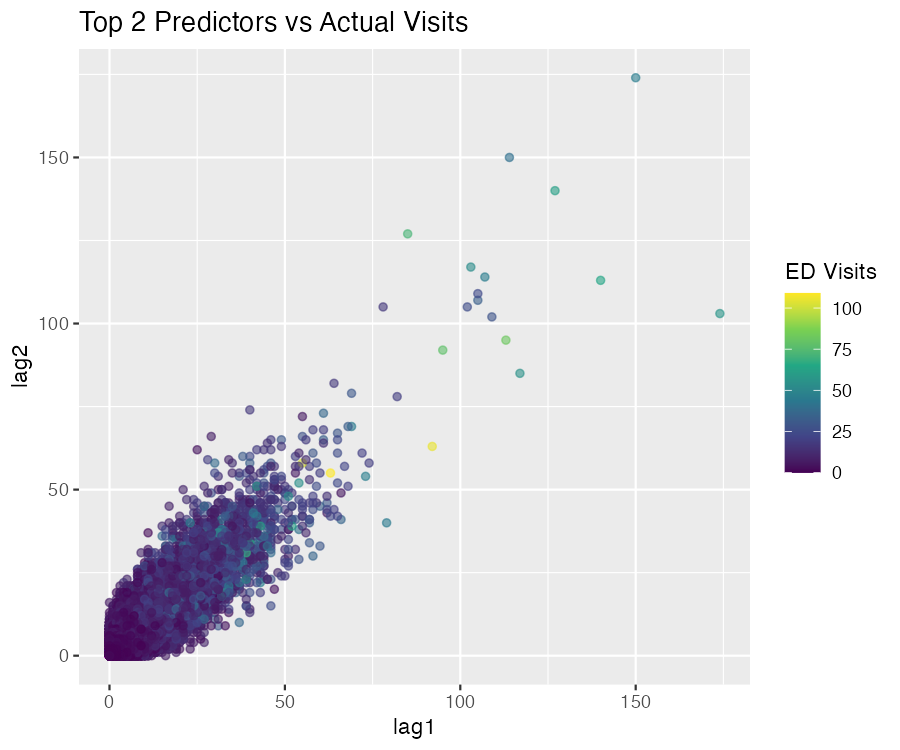
\includegraphics[width=\textwidth]{plot_actual_vs_top2.png}
    \subcaption{Actual visits \(y_{T+14}\) vs top two features}
  \end{minipage}\hfill
  \begin{minipage}[b]{0.32\textwidth}
    \centering
    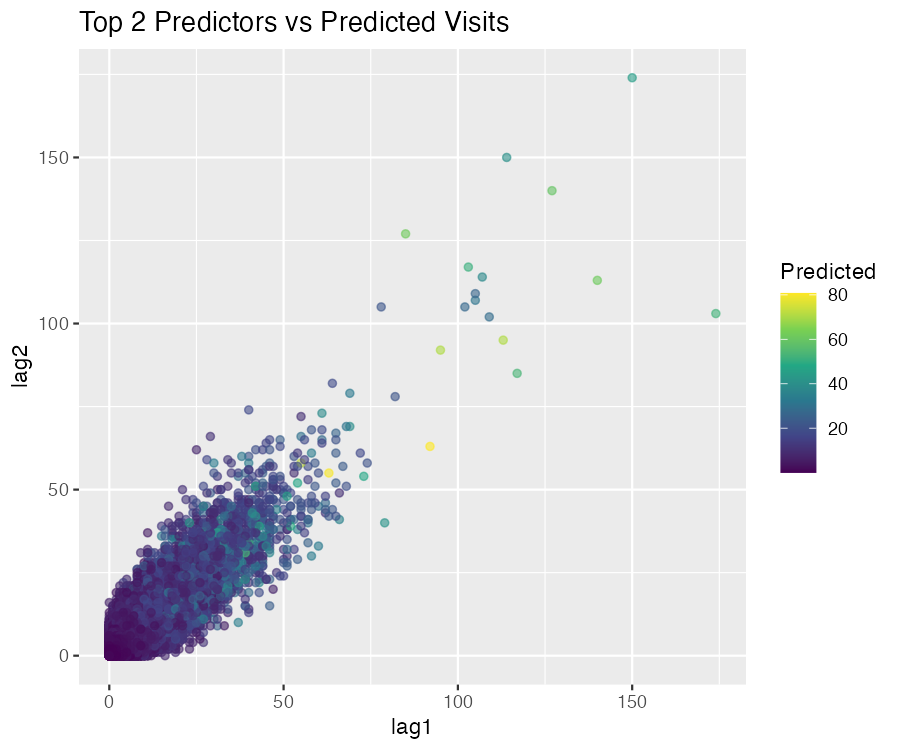
\includegraphics[width=\textwidth]{plot_predicted_vs_top2.png}
    \subcaption{Predicted visits vs top two features}
  \end{minipage}\hfill
  \begin{minipage}[b]{0.32\textwidth}
    \centering
    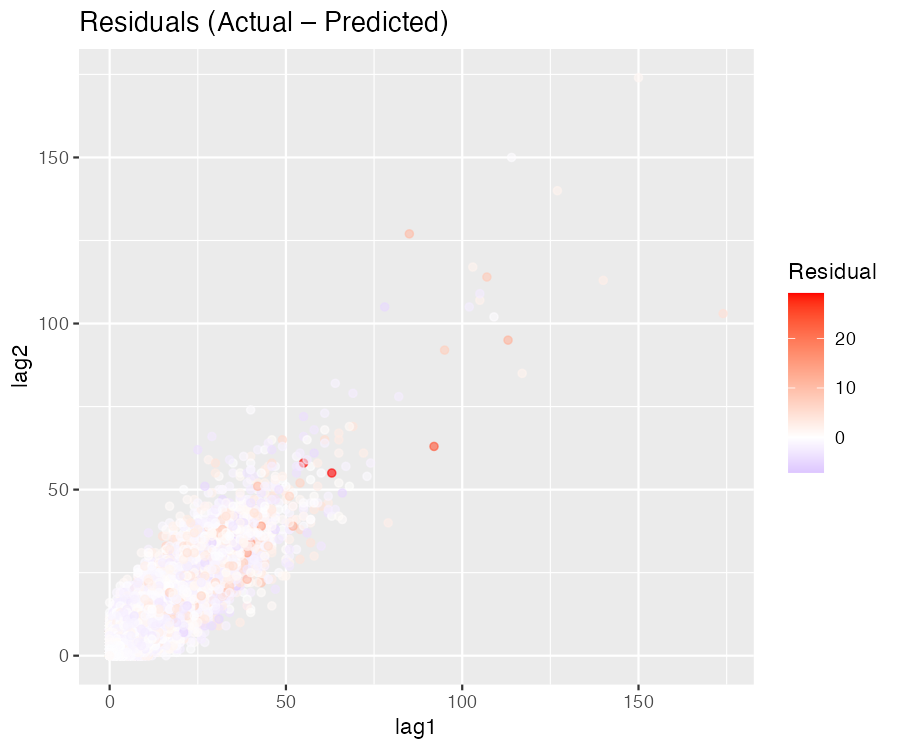
\includegraphics[width=\textwidth]{plot_residuals_vs_top2.png}
    \subcaption{Residuals (Actual–Predicted) vs top two features}
  \end{minipage}
  \caption{Scatterplots of the two most important predictors (lag1, lag2), colored by actual \(y\), predicted \(\hat y\), and residuals, respectively.}
  \label{fig:explore_top2}
\end{figure}

Comparing the actual and predicted visits plot, while the prediction shows very similar pattern to the actual values, when lag1 and lag2 are big, it over predicts the value. Also, the residuals also show some points that are extremely off the actual values. These show that some feature engineering that capture the pattern may be necessary.


\subsection{Feature Engineering}

I augmented our data with:

\begin{itemize}[nosep]
  \item \textbf{Total ED load.}  The overall ED visits that day, capturing system‐wide pressure and days with high volumes  
  \item \textbf{Extreme‐weather flags.}  Binary indicators for freezing days (\(\mathtt{temp<32°F}\)), heatwaves (\(\mathtt{temp>85°F}\)), rain, and high wind.  
  \item \textbf{Interaction term.}  \(\mathtt{cold\_and\_windy}\) to capture compounded respiratory stress.  
  \item \textbf{Binned temperature.}  5°F intervals, allowing piecewise effects.  
\end{itemize}

These are merged into \texttt{df\_feats\_model}, yielding 36 predictors plus the response. And the \texttt{rf\_cv\_feat} was trained using this new model.

\subsection{Time-Series Cross-Validation Comparison}

To understand how each new feature contributes to forecasting accuracy, I compared two random forest models using a realistic, forward-looking evaluation:

\begin{itemize}[nosep]
  \item \textbf{Baseline model:} trained on the two-week lagged ED visit counts plus raw weather variables.
  \item \textbf{Enhanced model:} trained on the same inputs \emph{plus} our engineered features (total ED load, extreme-weather flags, and interaction terms).
\end{itemize}

I evaluated both models with \emph{rolling-origin cross-validation}, which mimics real deployment by always training on past data and testing on the immediately following two-week window. Unlike random splits, rolling-origin validation trains only on dates strictly earlier than the test period, ensuring that each fold truly simulates a live forecasting scenario. It provides a robust estimate of how the model will perform in practice when making two-week-ahead predictions on unseen data. This procedure respects the time order and prevents peeking into the future.



\section{Results}

\subsection{Enhanced Model Diagnostics}

Figure~\ref{fig:enhanced_top2} displays the same three views—actual, predicted, and residual—this time for the enhanced model with engineered features:

\begin{figure}[H]
  \centering
  \begin{minipage}[b]{0.32\textwidth}
    \centering
    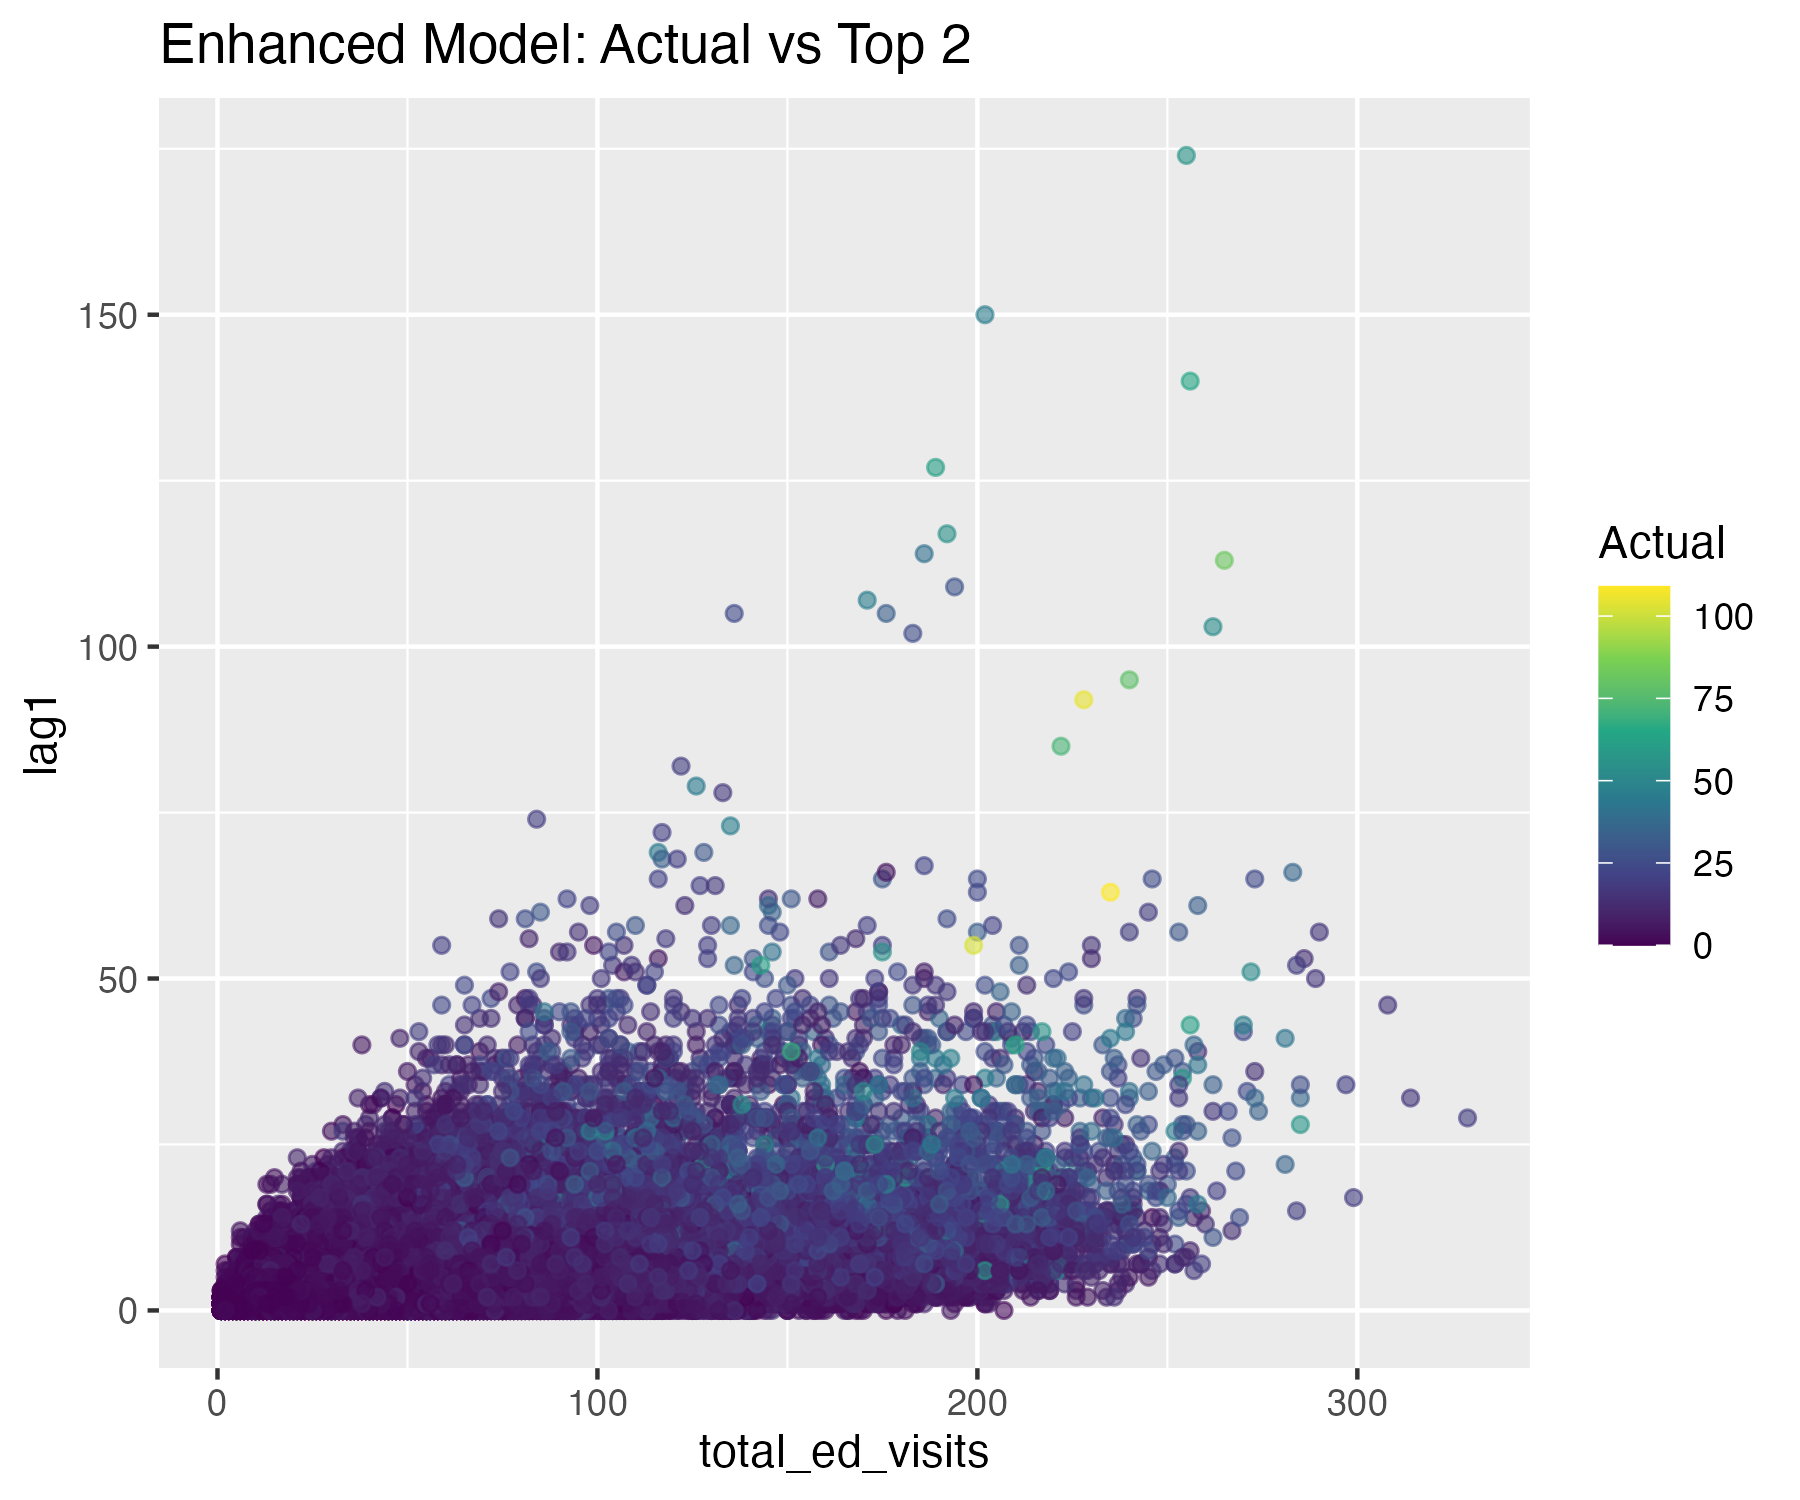
\includegraphics[width=\textwidth]{plot_actual_vs_top2_enhanced.png}
    \subcaption{Actual visits vs top two features}
  \end{minipage}\hfill
  \begin{minipage}[b]{0.32\textwidth}
    \centering
    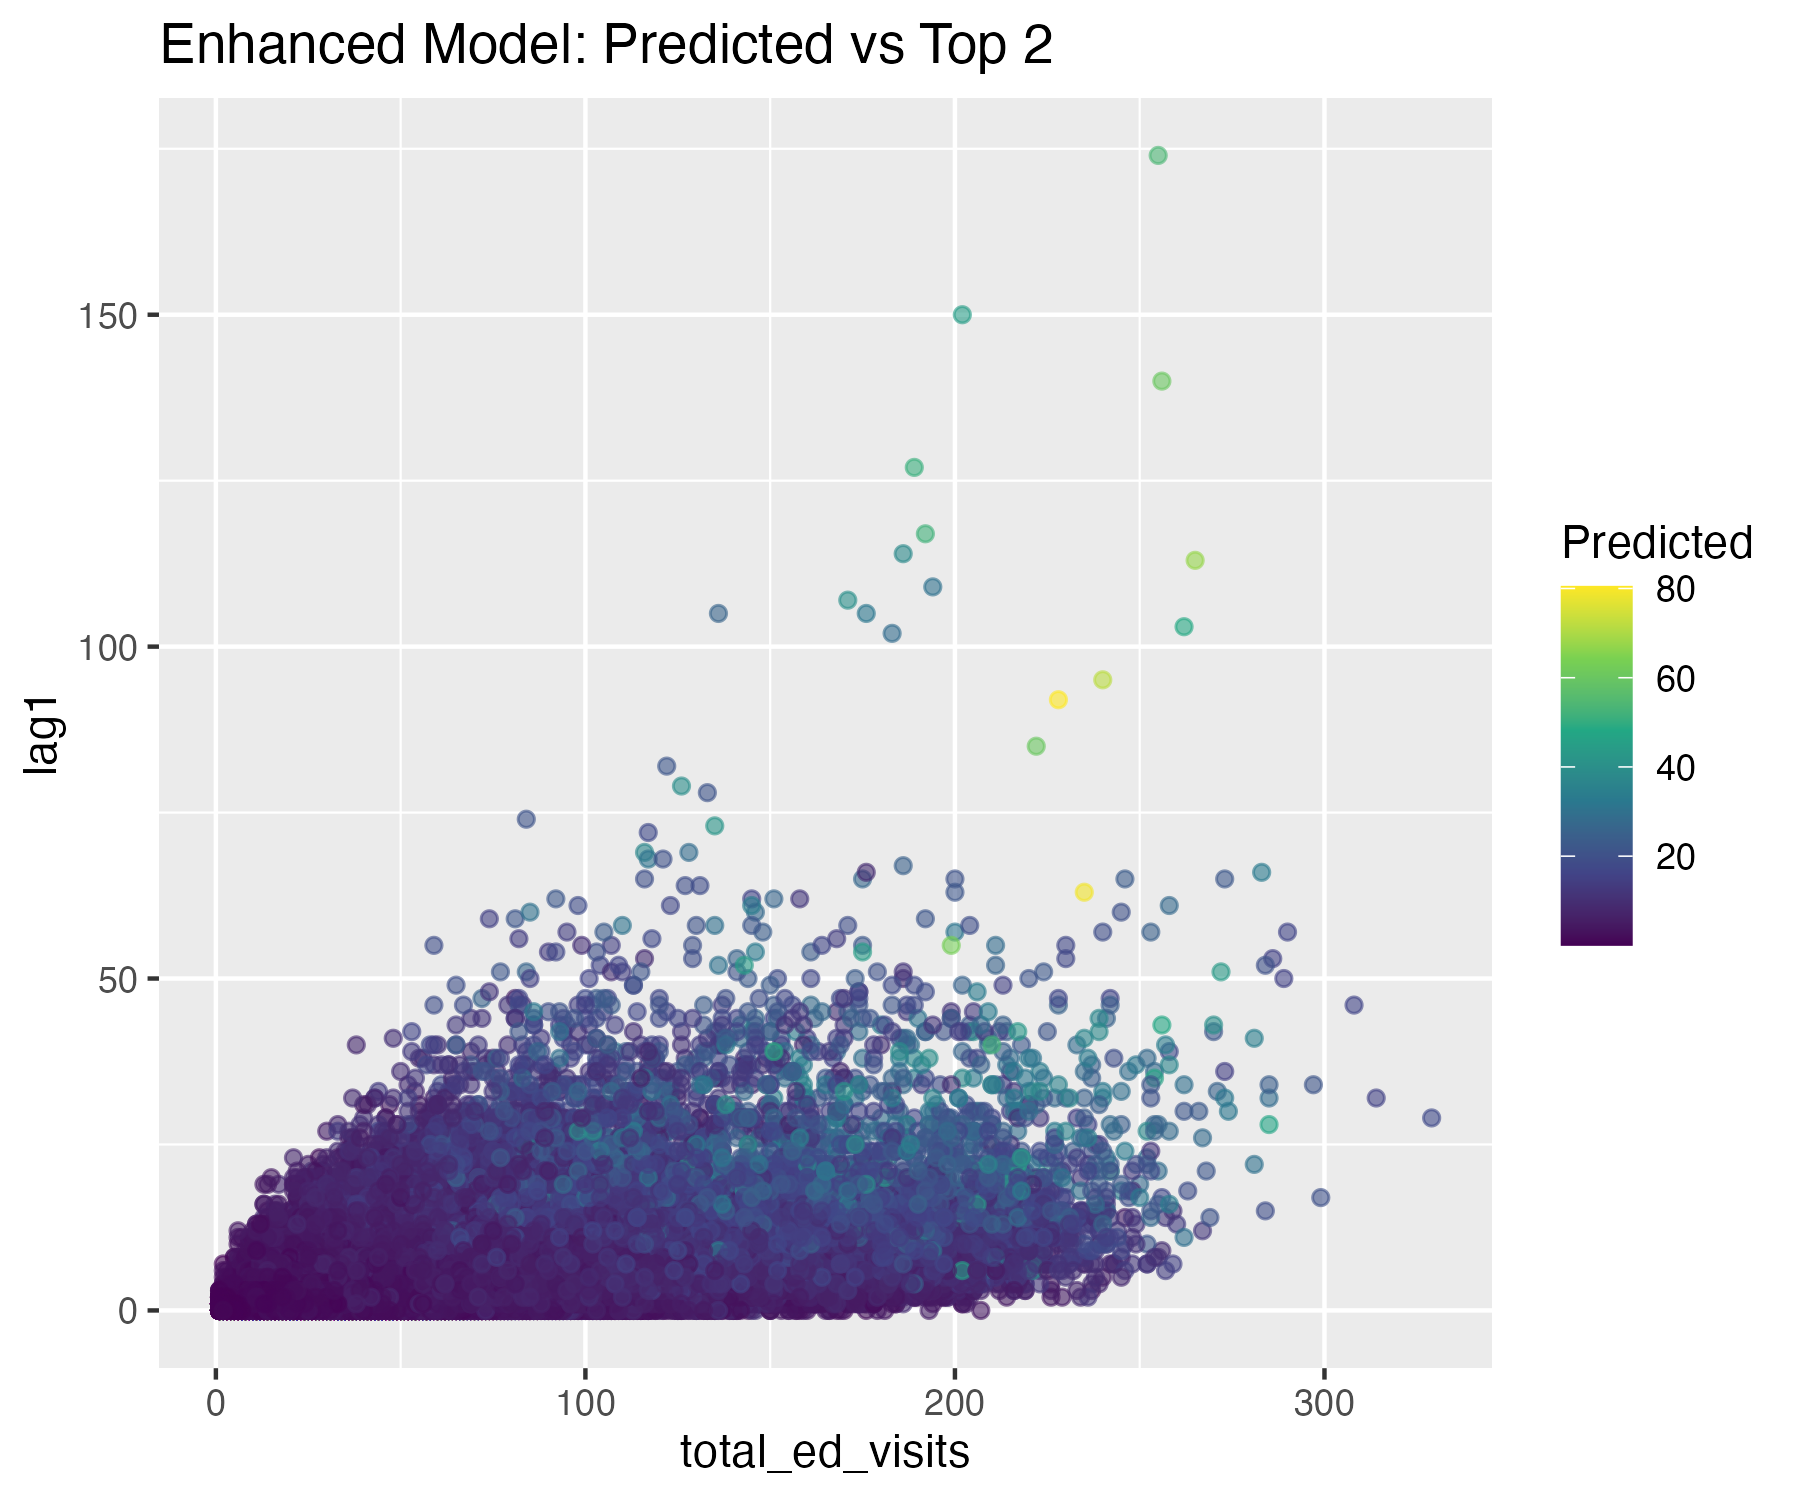
\includegraphics[width=\textwidth]{plot_predicted_vs_top2_enhanced.png}
    \subcaption{Predicted visits vs top two features}
  \end{minipage}\hfill
  \begin{minipage}[b]{0.32\textwidth}
    \centering
    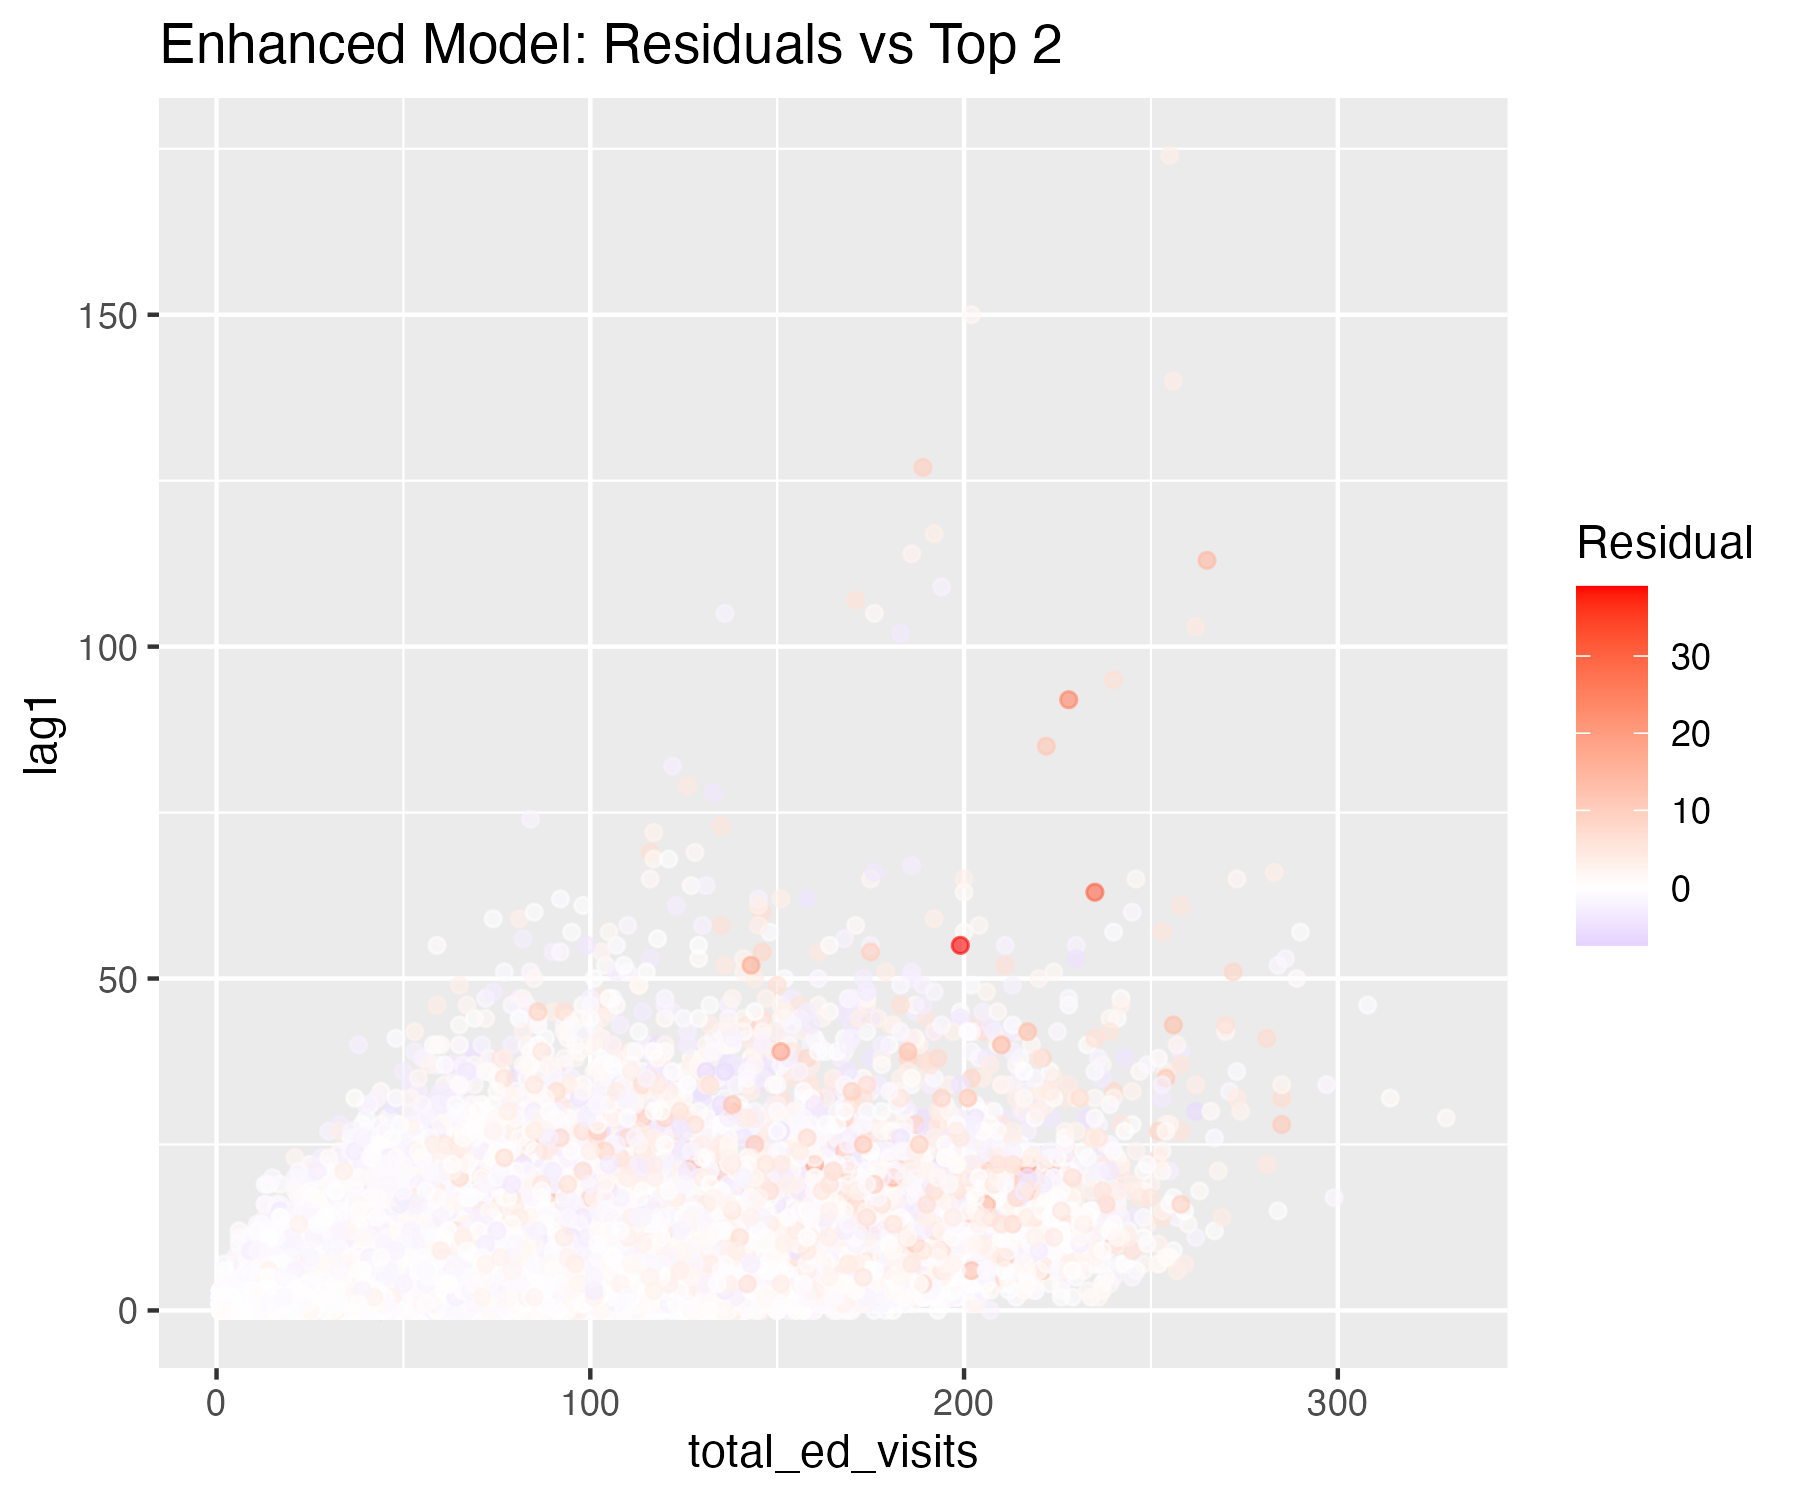
\includegraphics[width=\textwidth]{plot_residuals_vs_top2_enhanced.png}
    \subcaption{Residuals vs top two features}
  \end{minipage}
  \caption{Enhanced model diagnostics in the space of the two most important predictors.}
  \label{fig:enhanced_top2}
\end{figure}

Compared to the baseline model (Figure~\ref{fig:explore_top2}), the enhanced model’s predicted and actual plots are almost identical even in high lag1 and lag2 unlike the raw model without engineered features.
Also, the residual plot shows a fewer deep red dot indicating that the engineered features have helped correct the largest forecast error (failed with the one case). Also, the spread of residuals is more evenly dispersed across the feature plane, suggesting the model now captures the nonlinear interactions more completely. These diagnostics confirm that the targeted feature engineering addressed the systematic biases identified in the baseline model and materially improved predictive accuracy in those challenging regions of the feature space.  

After time-series cross-validation, the baseline model (lags + weather) achieved:
\begin{itemize}[nosep]
  \item Baseline CV RMSE: 2.40 visits
\end{itemize}

With engineered features added (total ED load, extreme-weather flags, interaction term), the enhanced model achieved:
\begin{itemize}[nosep]
  \item Enhanced CV RMSE: 2.39 visits
\end{itemize}

\noindent The enhanced model reduces the average two-week forecast error by approximately 0.01 visits. This is a small but measurable improvement given the low baseline error.  This confirms that our additional features capture subtle patterns (for example, days when total ED load and severe weather coincide) that pure lag-and-weather inputs miss.

On a held-out test set (last four weeks), final performance was:
\begin{itemize}[nosep]
  \item Hold-out RMSE: 4.81 visits
  \item Hold-out MAE: 3.00 visits
  \item Hold-out R\textsuperscript{2}: 0.70
\end{itemize}

\noindent These results confirm that our approach—leveraging two-week lagged counts, meteorological forecasts, and targeted engineered features—delivers sufficiently accurate predictions to inform proactive ED staffing and resource allocation in real operational settings.  

Figure~\ref{fig:holdout_residuals} summarizes residual diagnostics on the test set.

\begin{figure}[H]
  \centering
  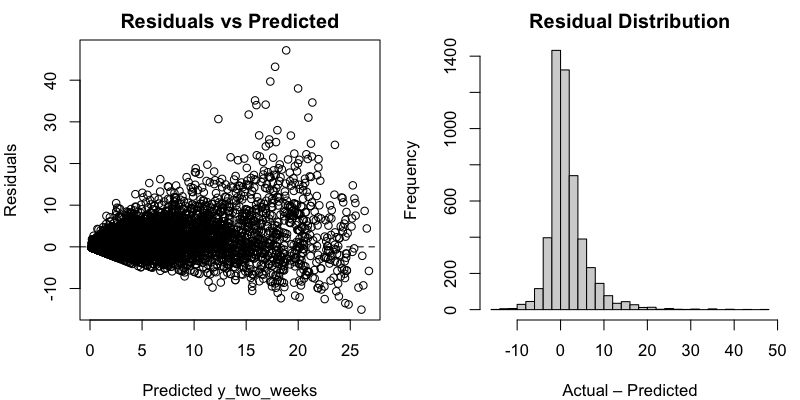
\includegraphics[width=\textwidth]{holdout_residuals.png}
  \caption{Left: Residuals vs Predicted for the hold-out set. Right: Distribution of residuals (Actual - Predicted).}
  \label{fig:holdout_residuals}
\end{figure}

The residuals are roughly centered around zero, with larger variance at high predicted volumes, and a right-skewed distribution indicating occasional under-predictions on spike days.

\section{Limitations and Risks}

Out‐of‐bag error tends to be optimistic because each tree’s OOB predictions still draw on information from the overall training sample; indeed, our true hold‐out RMSE (4.81 visits) was substantially higher than the OOB RMSE (2.53 visits), highlighting the bias inherent in this internal estimate. Moreover, I treated the Open‐Meteo 16 day forecasts as if they were perfect when predicting two weeks ahead. In practice, meteorological forecasts carry their own error which will propagate through our model and degrade real‐world performance, especially during extreme weather events.

My feature set is by design limited to meteorological variables and recent ED visit lags. I do not incorporate other important drivers such as air quality, public holidays, school calendars, or local outbreak reports. Omitting these factors may leave systematic demand surges unexplained and reduce accuracy during periods when non‐weather influences dominate patient behavior.

When I examine the residuals, I observe heteroscedasticity: variance grows with predicted volume, so error bars widen on high‐demand days. This suggests the potential benefit of variance stabilizing transforms or probabilistic forecasting methods to explicitly model and communicate uncertainty. Finally, several test days recorded zero ILI/pneumonia visits, making percentage‐based metrics (like MAPE) undefined and causing models tuned on MAE/RMSE to underweight performance at the low end of the demand spectrum. Trained exclusively on NYC data from 2020–2022, our model may also have limited generalizability to other seasons (e.g.\ post‐pandemic dynamics), different climate regimes, or non‐respiratory ED demands.


\section{Conclusion}

In this project, I addressed the critical operational problem of predicting two‐week–ahead ED visits for influenza‐like illness and pneumonia, enabling hospital administrators to shift from reactive staffing to proactive resource allocation. My most striking result is that the enhanced random forest model that combined combined two-week lagged visit counts, historical and forecasted weather, and targeted engineered features—achieves a hold‐out MAE of 3.0 visits and explains 70 \% of the day-to-day variance.  

Using two large, complementary datasets which are a 2.5-year daily record of ED visits across 177 NYC ZIP codes (176 862 × 5) and matched historical plus 16-day forecast weather data (181 248 × 18), I built a model capable of capturing both autoregressive trends and complex meteorological interactions. I compared four feature sets via OOB error and time-series CV, demonstrating that the combined approach outperforms lag-only or weather-only baselines.  

My approach was chosen for its balance of accuracy, interpretability, and computational efficiency: random forests handle correlated predictors without aggressive dimensionality reduction, naturally accommodate nonlinear interactions (e.g.\ cold + windy flags), and provide internal error estimates via OOB.  Alternative methods such as linear regression, ARIMA, or purely autoregressive trees would've lacked either predictive power or flexibility in incorporating forecast inputs.

Key limitations include optimistic OOB estimates, unmodeled forecast uncertainty, omitted covariates (air quality, holidays), and heteroscedastic errors on peak days. These suggest future enhancements such as variance‐stabilizing transforms and integration of non‐weather drivers.  

Overall, this work establishes a robust, data‐driven early‐warning system that predicts ED respiratory demand to within ±3 visits, two weeks in advance.  By translating weather forecasts into actionable staffing projections, the model has the potential to reduce wait times, prevent resource bottlenecks, and ultimately improve patient outcomes during seasonal illness surges.  

\end{document}
